\documentclass[usenames,dvipsnames]{beamer}


\usepackage{minted}
\usepackage{xcolor}
\usepackage{amsmath}

\usepackage{float}
\usepackage{graphicx}
\usepackage{nicefrac}
\usepackage{microtype}
\usepackage[minmargin=0.1\hsize,labelfont=bf, labelsep=period]{caption}
\usepackage{fancyvrb}
\usepackage{appendixnumberbeamer}
\usepackage{tikz}
\usetikzlibrary{
  decorations.pathreplacing,
  calc,
  patterns}

%%% fonts
\usefonttheme[onlymath]{serif}
\usepackage{mathpple}

\usepackage[light]{iwona}
\usepackage[T1]{fontenc}

%%% beamer commands
\setbeamertemplate{navigation symbols}{}  % remove nav icons
\useoutertheme{split}
\usetheme{Boadilla}
\usecolortheme[named=RoyalBlue]{structure}
\setbeamertemplate{blocks}[default]

%%% DW's commands
\renewcommand{\vec}{\boldsymbol}
\newcommand{\makeTimeEventTable}{%
\begin{tabular}{rl}
         Time        &  Event indicator  \\
                     &                   \\
     \Large  $T_i$   & \Large $\delta_i$ \\
                     &                   \\
           24        &      1            \\
%          11        &      0            \\
           93        &      0            \\
           43        &      1            \\
           43        &      0            \\
           \vdots    &                   \\
           39        &      1            \\
\end{tabular}}

\title[Likelihood and measurement]{Likelihood and measurement}
\subtitle{Modelling approaches for real data}
\author{Dirk Bester}
\date{2023-10-02}

\begin{document}

\begin{frame}
\maketitle
\end{frame}

\section{Introduction}

\subsection{Intro}

\begin{frame}[t]
  \tableofcontents[currentsubsection]
\end{frame}

\begin{frame}[t]
\frametitle{Introduction}
\begin{center}

\end{center}
\begin{block}{\textbf{Measurement}}
``Most neglected subject in all of statistics.''
\\
\hfill {\small Andrew Gelman}
\end{block}

\pause
Simply, \textit{how} you observe influences \textit{what} you observe.

\pause
Less simply, the measurement process is as important as the data-generating process.
People often just ignoring it.
\pause
Well known example: people like to round numbers

\pause
This influences how the likelihood is constructed.

\end{frame}


\subsection{Problem statement}

\begin{frame}[t]
  \tableofcontents[currentsubsection]
\end{frame}

\begin{frame}[t]
\frametitle{Problem statement}

We want to sell Cyber security insurance.
\pause \\
Data is scarce.
Companies aren't willing to share data with each other.
\pause \\
One consulting firm collected information from a set of their clients and published it in aggregated form.
(See next slide for details).

\pause \vfill

Companies were happy for their data to be shared this way, because how could it possibly be useful to their competitors...

\end{frame}

\begin{frame}[t]
\frametitle{Problem statement}

I have this data for 2013, 2014, 2015:

\footnotesize
\begin{tabular}{|l|r|r|r|r|r|r|}
\hline
Business.Sector & Claims & Min & Median & Mean & Max & year\\
\hline
Education & 8 & 2560 & 132650 & 204858 & 680000 & 2013\\
\hline
Entertainment & 2 & 1125000 & 5812500 & 5812500 & 10500000 & 2013\\
\hline
Financial Services & 8 & 20100 & 166000 & 1060138 & 4750000 & 2013\\
\hline
Healthcare & 29 & 5390 & 254000 & 1612343 & 20000000 & 2013\\
\hline
  \ldots   &    &      &        &  \ldots &          &     \\
\hline
  \ldots   &    &      &        &  \ldots &          &     \\
\hline
Professional Services & 10 & 6704 & 29217 & 329845 & 2989966 & 2015\\
\hline
Restaurant & 5 & 4000 & 16212 & 75744 & 250000 & 2015\\
\hline
Retail & 12 & 91359 & 455488 & 1795266 & 8916432 & 2015\\
\hline
Technology & 11 & 0 & 90000 & 206532 & 641635 & 2015\\
\hline
Other & 15 & 708 & 61339 & 713133 & 6700142 & 2015\\
\hline
\end{tabular}
\normalsize
... and I want to fit this model:
\begin{align*}
 y   &\sim GLM( g^{-1}( X \beta) ) \\
\only<1>{
     &\sim Dist( \text{mean} = g^{-1}( X \beta) , \text{variance} ) \\
     }
\only<2>{
 y_i &\sim LogNormal( \text{mean} = \exp{( \alpha + \beta_{year_i} +  \beta_{sector_i})} , \text{variance} ) \\
 y_i &\sim Pareto( \text{mean} = \exp{( \alpha + \beta_{year_i} +  \beta_{sector_i})} )
 }
\end{align*}


\end{frame}


\subsection{Quick jargon}

\begin{frame}[t]
\frametitle{Industry problem: Jargon}
\begin{center}
\begin{tabular}{rl}
\Large $y$             & $\Large \vec{x} = \{x_1, x_2 \ldots x_k \}$     \\
                       &                                 \\
\structure<2->{Variate}   & \structure<2->{Covariate}          \\
                       &                                 \\
Dependent variable     & Independent variable            \\
Outcome                & Predictor                       \\
Explained              & Explanatory                     \\
Regressand             & Regressor                       \\
Response variable      & Controlled variable             \\
Endogenous             & Exogenous                       \\
Experimental variable  & Manipulated variable            \\
                       & Exposure variable               \\
                       & Risk factor                     \\
Studied variable       & Measured variable               \\
Target                 & Feature                         \\
Output                 & Input                           \\
\end{tabular}
\end{center}
\end{frame}



\section{Likelihood construction and measurement}

\subsection{Definition}

\begin{frame}[t]
  \tableofcontents[currentsubsection]
\end{frame}


\begin{frame}[c]
    \frametitle{Formal definition}
    \centering
    A function that includes the \structure{data and the parameters} that is \structure{proportional} to the \structure{probability} of observing the data.
    \begin{align*}
    {\mathcal {L}}(\theta ; x)
    &\propto
    P_\theta(X=x) \uncover<3->{ \qquad \text{(Frequentist)} } \\
    \uncover<2->{
    &=
    P(X=x \;\vert\; \theta)
    \text{.}
    \uncover<3->{ \qquad \text{(Bayesian)} }
    }
    \end{align*}
\end{frame}

\begin{frame}[t]
    \frametitle{Formal definition}
    {
    \Large
    Discrete
    }
    \begin{align*}
    {\mathcal {L}}(\beta ; x)
    &\propto
    P_\beta(X=x) \\
    &=
    f_\beta(x)
    \end{align*}
    \pause
    {
    \Large
    Continuous
    }
    \begin{align*}
    {\mathcal {L}}(\beta ; x)
    &\propto
    P_\beta(X=x) \\
    &=
    P_\beta(x <  X\leq x + dx) \\
    &=
    f_\beta(x) dx \\
    &\propto
    f_\beta(x)
    \end{align*}
    \pause
    {
    \Large
    $n$ i.i.d. observations
    }
    \begin{align*}
    {\mathcal {L}}(\beta ; x)
    =
    \prod_{i}^{n}{
    f_\beta(x_i)
    }
    \end{align*}
\end{frame}


\subsection{Measurement: Truncation}

\begin{frame}
\frametitle{Measurement}
\begin{block}{Truncation}
Under certain conditions, you don't see anything.
\end{block}

Example: You only see events if they occur after $c= 30$ days.

\textbf{Likelihood contribution} for event at time $t$.
\begin{center}
\begin{tabular}{|p{2cm}|p{2cm}|}
   \hline
   Pure          & Truncation present \\
   \hline
                 &            \\
   $f(t)$ & $\displaystyle \frac{ f(t) }{1-F(30)} $ \\
                 &            \\
   \hline
\end{tabular}

\vfill
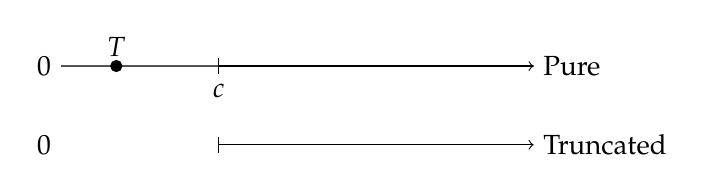
\begin{tikzpicture}
  \filldraw (0,0) node[left] (start) {$0$} --
  (0.7,0) circle (2pt)node[above] (beforeend) {$T$} --
  (6,0) node (end) {} ;
  \draw[->] (2,0)  -- (6,0) node[right] {Pure};
  \draw (2,-0.1) node[below] {$c$} -- (2,0.1)  ;

  \begin{scope}[yshift=-1cm]
  \node at (0,0) [left] (start) {$0$};
  \draw[->] (2,0)  -- (6,0) node[right] {Truncated};
  \draw (2,-0.1) -- (2,0.1);
\end{scope}
\end{tikzpicture}


\end{center}

\end{frame}

\subsection{Measurement: Censoring}
\begin{frame}
\frametitle{Measurement}

\begin{block}{Censoring}
Under certain conditions, you only get limited information.
\end{block}

Example: You only have data for a 10 year window. If you don't see an event in this period, you know it occurs at $T>10$.

\textbf{Likelihood contribution} for no event in your period of 10 years (the real event happened, say, at time 12.)
\begin{center}
\begin{tabular}{|p{4cm}|p{4cm}|}
   \hline
   Pure         & Censoring present \\
   \hline
                 &            \\
   $f(12)$ & $P(T > 10) = S(10)$ \\
                 &            \\
   \hline
\end{tabular}

\vfill
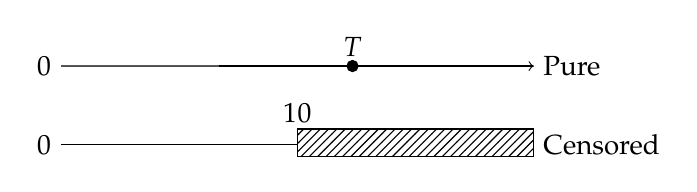
\begin{tikzpicture}
  \filldraw (0,0) node[left] (start) {$0$} --
  (3.7,0) circle (2pt)node[above] (beforeend) {$T$} --
  (6,0) node (end) {} ;
  \draw[->] (2,0)  -- (6,0) node[right] {Pure};

  \begin{scope}[yshift=-1cm]
  \filldraw (0,0) node[left] (start) {$0$} -- (3,0) ;
  \node at (6,0) [right] {Censored};
  \draw[pattern= north east lines] (3,-0.15) rectangle (6,0.2);
  \node at (3,0.15) [above] {$10$};
  \end{scope}
\end{tikzpicture}

\end{center}
\end{frame}



\subsection{Our example}

\begin{frame}
\frametitle{Our example}
\begin{align*}
\text{stddev}   &= cv \times \text{mean} \\
\sigma^2 &=  \log( 1+( \text{stddev}^2 )/( \text{mean}^2 ) )   \\
\mu    &= \log( \text{mean} ) - \frac{1}{2} \sigma^2
\text{.}
\end{align*}
Hence the following is equivalent:
\begin{align*}
 y \sim \text{lognormal2}&( \text{mean}_i, cv) \\
 y \sim \text{lognormal} &\bigg(
 \mu    = \log( \text{mean} ) - \frac{1}{2}
           \log( 1+( (cv \times \text{mean})^2)/( \text{mean}^2 ) )^2
   , \\
 &\sigma^2 = \log( 1+( cv \times \text{mean}^2)/( \text{mean}^2 ) )
 \bigg)
 \text{.}
\end{align*}

That is, we have reparametrised the lognormal distribution so that we can think in terms of its mean and coefficient of variation, instead of the unintuitive $\mu$ and $\sigma$.


\end{frame}


\begin{frame}

If we have a random variable $X_i$, independently and identically distribution, with a cumulative distribution function (CDF) $F(x)$ and a density $f(x)$, we can derive the distribution of
$Y = \operatorname{max}\big(\{ X_1 , X_2 , X_3 , \ldots, X_n \} \big)$,
\begin{align*}
F_Y(x) &= P\left( \operatorname{max}\big(\{ X_1 , X_2 , X_3 , \ldots, X_n \} \big) < x \right) \\
   &= P\left( \text{all } X_i \text{ less than } x \right) \\
   &= P\left( X_1 < x, X_3 < x, X_3 < x, \ldots, X_n < x \right) \\
   &=   P( X_1 < x)
        P( X_2 < x)
        P( X_3 < x)
       \ldots
        P( X_n < x) \\
   &=   \prod_{i=1}^{n}{ P( X_i < x)} \\
   &=   \prod_{i=1}^{n}{ F_X(x) } \\
   &=   \left( F_X(x) \right)^n
\end{align*}

and thus
\begin{align*}
f_Y(x)
&= \frac{d}{dx}  \left( F_X(x) \right)^n  \\
&= n \left( F_X(x) \right)^{n-1} f_X(x)
\text{.}
\end{align*}

\end{frame}



\begin{frame}

We can do the same for the minimum of a set of observations, or for any order statistic%
\footnote{\href{https://en.wikipedia.org/wiki/Order_statistic}{\texttt{https://en.wikipedia.org/wiki/Order\_statistic}}}
Let $X_{(k)}$ be the $k$th order statistic, then
\begin{align*}
f_{X_{(k)}}(x) &=
\frac{n!}{(k-1)!(n-k)!} [F_X(x)]^{k-1} [1- F_X(x)]^{n-k} f_X(x)
\text{.}
\end{align*}

We can also write down the joint distribution for pairs of order statistics!
For the pair of order statistics%
\footnote{
\href{https://en.wikipedia.org/wiki/Order_statistic\#The_joint_distribution_of_the_order_statistics_of_an_absolutely_continuous_distribution)
}{
\texttt{https://en.wikipedia.org/wiki/Order\_statistic}
}
}
$( X_{(j)} , X_{(k)} )$
from $n$ observations, the joint distribution is:
\begin{align*}
f_{X_{(j)} , X_{(k)} }(x, y) &=
\frac{n!}{(j-1)!(k-j-1)!(n-k)!} \times \\
&
[F_X(x)]^{j-1}
[F_X(y) - F_X(x)]^{k-1-j}
[1 - F_X(x)]^{n-k}
f_X(x)
f_X(y)
\end{align*}


\end{frame}


\begin{frame}
\small
Let's carry on.
For the three order statistics.
Their distribution is
\begin{align*}
f_{X_{(j)} , X_{(k)}, X_{(l)}  }(x, y, z) = &
\quad
\text{\structure{Big Ugly Equation}}
\\
&
\frac{n!}{ (j-1)! (k-j-1)! (l-k-1)! (n-k)! } \\
& \times
[F_X(x)]^{j-1}
[F_X(y) - F_X(x)]^{k-j-1}
\\
& \times
[F_X(z) - F_X(y)]^{l-k-1}
[1 - F_X(z)]^{n-l} \\
& \times
f_X(x)
f_X(y)
f_X(z)
\end{align*}

\end{frame}



\section{Model}

\subsection{Likelihood}

\begin{frame}[t]
  \tableofcontents[currentsubsection]
\end{frame}



\begin{frame}
\frametitle{Conclusion: Measurement and Likelihood}
Each row in our dataset can be thought of as an observation from a joint distribution.
For row $i$ we have
\begin{align*}
\boldsymbol{y}_i = \{y_{\text{min}}, y_{\text{med}}, y_{\text{max}}, n \}_i
\end{align*}
and its likelihood
\begin{align*}
{\mathcal {L}}(\theta ;\boldsymbol{y}_i)
&=
f_{X_{(1)} , X_{(n_i/2)}, X_{(n_i)}  }(y_{i\text{min}}, y_{i\text{med}}, y_{i\text{max}})
\end{align*}
and then we have the likelihood for all the data $D$ in the $N$ rows,
\begin{align*}
{\mathcal {L}}(\theta ; \boldsymbol{D})
&=
\prod_{i=1}^{N}{
f_{X_{(1)} , X_{(n_i/2)}, X_{(n_i)}  }(y_{i\text{min}}, y_{i\text{med}}, y_{i\text{max}})
}
\end{align*}


Recall that we believe our data to be from a process:
\begin{align*}
 y_i &\sim LogNormal( \text{mean} = \exp{( \alpha + \beta_{year_i} +  \beta_{sector_i})} , \text{variance} )
\end{align*}
so we will use $F(x)$ and $f(x)$ (the CDF and pdf) of the LogNormal distributoin to write down the \structure{Big Ugly Equation}.

\end{frame}


\subsection{Estimation}

\begin{frame}[t]
  \tableofcontents[currentsubsection]
\end{frame}

\begin{frame}
\frametitle{Estimation}

We can write down the likelihood. Now we just have to maximise it! How?

\begin{center}
\begin{tabular}{ccc}
\hline
Custom code &  ?   &Hard to debug, error prone \\
Tensorflow  &  python   &  requires ``hacks''  \\
Pytorch     &  python   &  requires ``hacks'' \\
statsmodels &  python   & GenericLikelihoodModel \\
PyMC        &  python   & syntax quite bad   \\
Stan        &  stan     & R + library(rstan)  \\
            &           & python + import cmdstanpy \\
\hline
\end{tabular}
\end{center}


A lot of the above make use of automatic differentiation libraries.
There are a lot of these out there as well.
Check which one is closest to what you are comfortable with.

\end{frame}

\begin{frame}[fragile]
\frametitle{Stan}

\centering
\href{https://mc-stan.org/docs}{https://mc-stan.org/docs}

\vfill
\tiny

R Code:
\begin{minted}[frame=lines]{R}
library(rstan)
theta <- 0.1
n <- 1000
y <- rexp(n, theta)
my_dat <- list(N = n, y = y)
fit <- stan(
    file = 'stanmodel.stan', 
    data = my_dat,  iter = 10000)
summary(fit)
plot(fit)
\end{minted}

Stan code:
\begin{minted}[frame=lines]{stan}
data {
  int<lower=0> N;
  vector[N] y;
}
  parameters {
  real<lower=0> theta;
}
model {
  y ~ exponential(theta);
  theta ~ lognormal(0, 1000);
}
\end{minted}

\end{frame}

\begin{frame}
\begin{columns}
\begin{column}[c]{0.49\textwidth}
   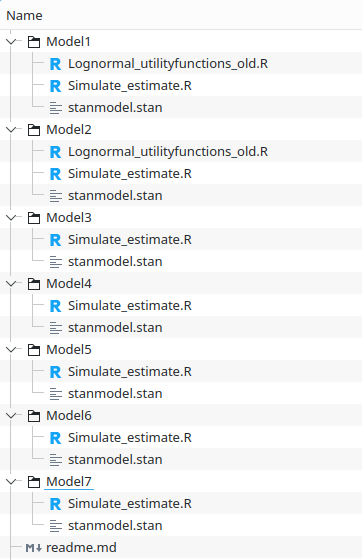
\includegraphics[width=0.50\textheight]{./plots/Model_testing}
\end{column}
\begin{column}[c]{0.40\textwidth}
Test the code by simulating real data and checking that we can estimate the true parameters.
Start simple add more and more complexity.
\end{column}
\end{columns}
\end{frame}



\subsection{Results}

\begin{frame}[t]
  \tableofcontents[currentsubsection]
\end{frame}


\begin{frame}
\begin{columns}
\begin{column}[c]{0.49\textwidth}
   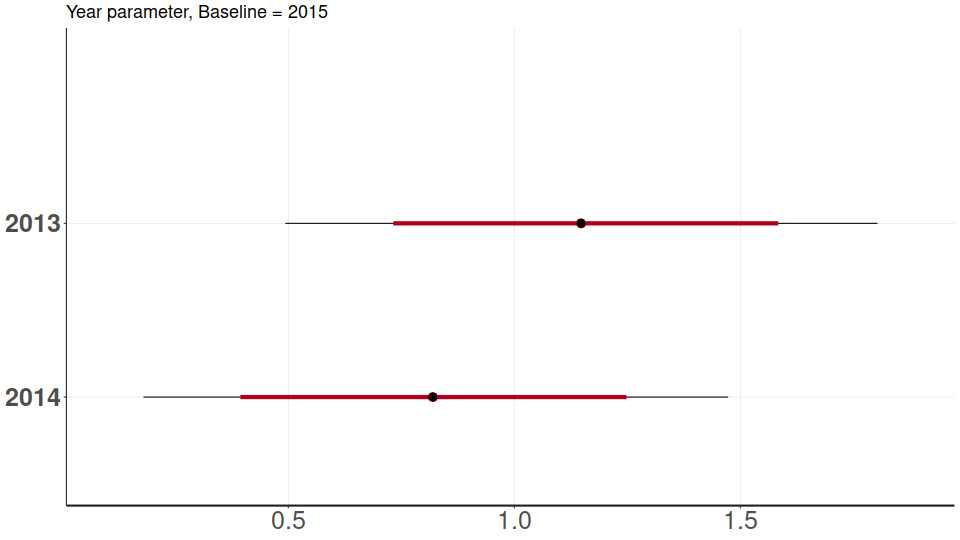
\includegraphics[width=0.60\textheight]{./plots/year_comparison}
\end{column}
\begin{column}[c]{0.49\textwidth}
   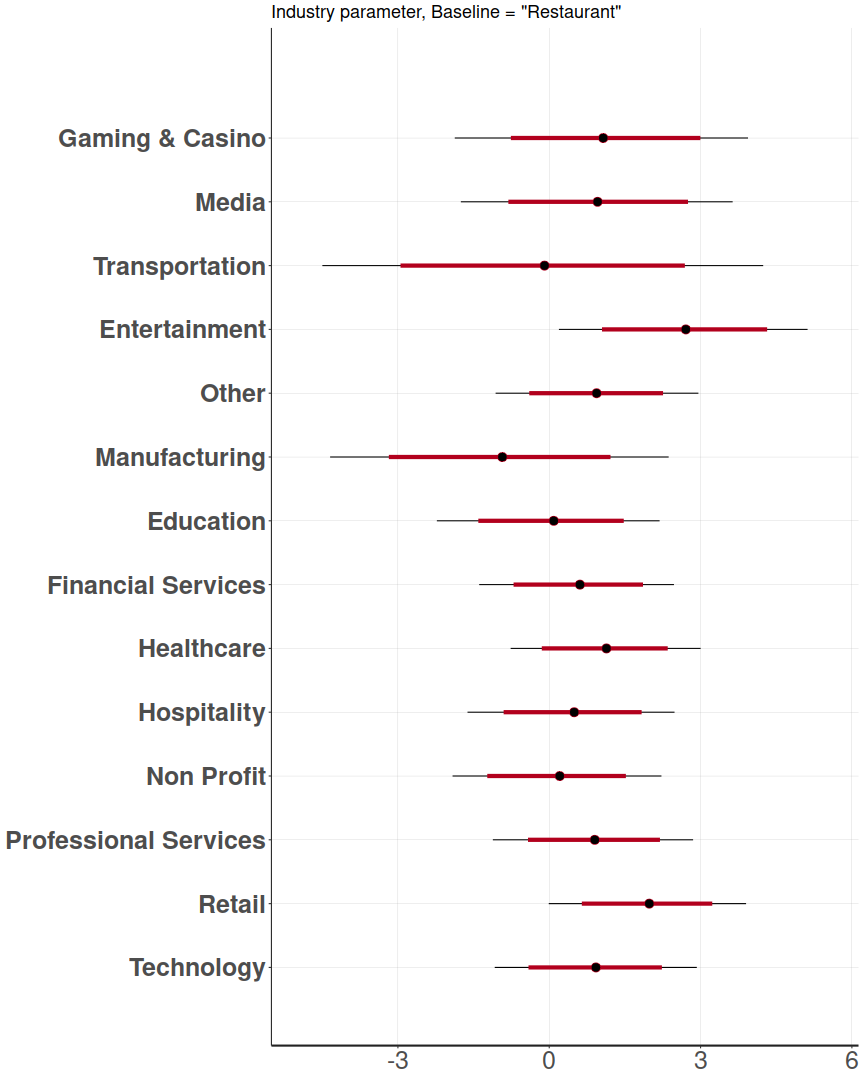
\includegraphics[width=0.60\textheight]{./plots/sector_comparison}
\end{column}
\end{columns}
\vfill
Recall that $y_i$ is the claim severity.
\begin{align*}
  y_i &\sim LogNormal( \text{mean} = \exp{( \alpha + \beta_{year_i} +  \beta_{sector_i})} , \text{variance} )
\end{align*}
\end{frame}


\begin{frame}
\begin{center}
   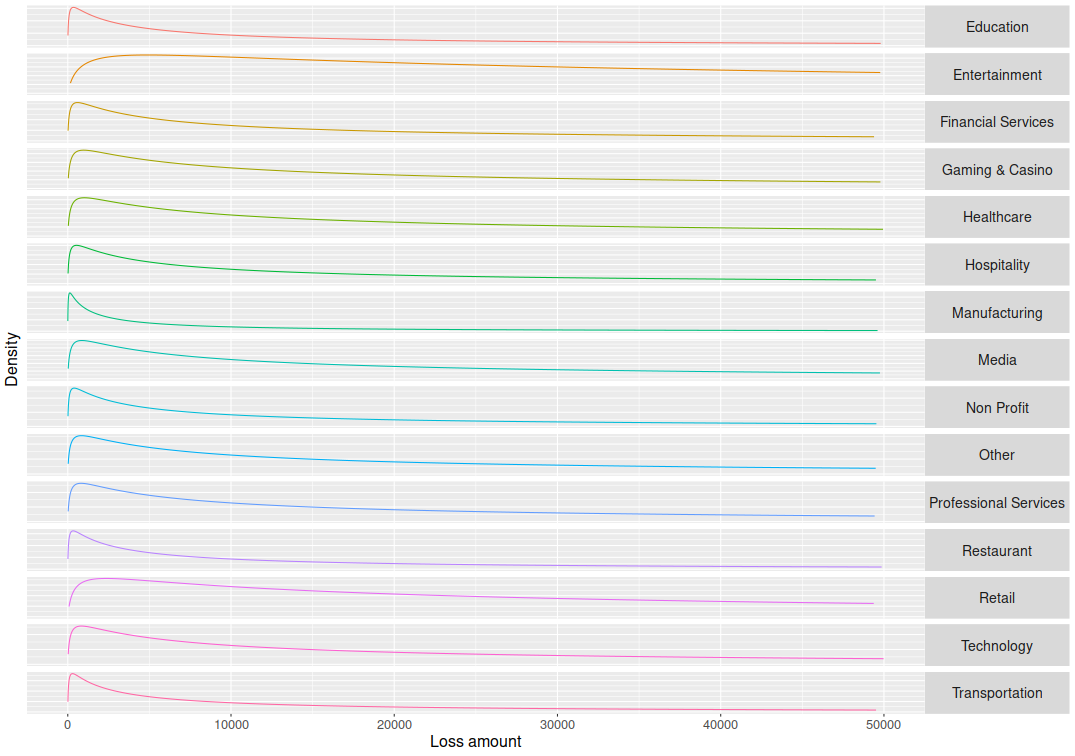
\includegraphics[width=1.2\textheight]{./plots/distplot}
\end{center}
\begin{align*}
  y_i &\sim LogNormal( \text{mean} = \exp{( \alpha + \beta_{year_i} +  \beta_{sector_i})} , \text{variance} )
\end{align*}
\end{frame}


\begin{frame}[fragile]

\tiny

\begin{minted}{r}
deductible <- 10e3
limit <- 10e6

payout <- function(x, deductible, limit){
  if (x < deductible)  return(0)
  else if (deductible <= x & x < limit )  return(x - deductible)
  else if (limit <= x )  return(limit - deductible )
}
payout <- Vectorize(payout, "x")

montecarlo_expected_claim <- function(mu, sigma, N=10000, deductible=deductible, limit=limit){
  sim_claim <- rlnorm(N, mu, sigma)  
  sim_payouts <- payout(sim_claim, deductible, limit)
  return(mean(sim_payouts))
}
\end{minted}



\begin{tabular}{|r|r|l|r|r|r|}
\hline
 sector & mean\_payout & claim\_frequency & premium\\
\hline
\hline
 Gaming \& Casino & 502,125 & 0.1 & 50,212.5\\ \hline
 Media & 435,513 & 0.1 & 43,551.3\\ \hline
 Transportation & 179,929 & 0.1 & 17,992.9\\ \hline
 Entertainment & 1,613,356 & 0.1 & 161,335.6\\ \hline
 Other & 449,043 & 0.1 & 44,904.3\\ \hline
 Manufacturing & 77,390 & 0.1 & 7,739.0\\ \hline
 Education & 195,717 & 0.1 & 19,571.7\\ \hline
 Financial Services & 327,431 & 0.1 & 32,743.1\\ \hline
 Healthcare & 519,231 & 0.1 & 51,923.1\\ \hline
 Hospitality & 291,054 & 0.1 & 29,105.4\\ \hline
 Non Profit & 238,819 & 0.1 & 23,881.9\\ \hline
 Professional Services & 418,962 & 0.1 & 41,896.2\\ \hline
 Retail & 1,032,428 & 0.1 & 103,242.8\\ \hline
 Technology & 432,961 & 0.1 & 43,296.1\\ \hline
 Restaurant & 202,587 & 0.1 & 20,258.7\\ \hline
\end{tabular}

 
\end{frame}


\end{document}

